\begin{figure*}[ht]
\centering
\begin{minipage}{0.9\textwidth}
\centering
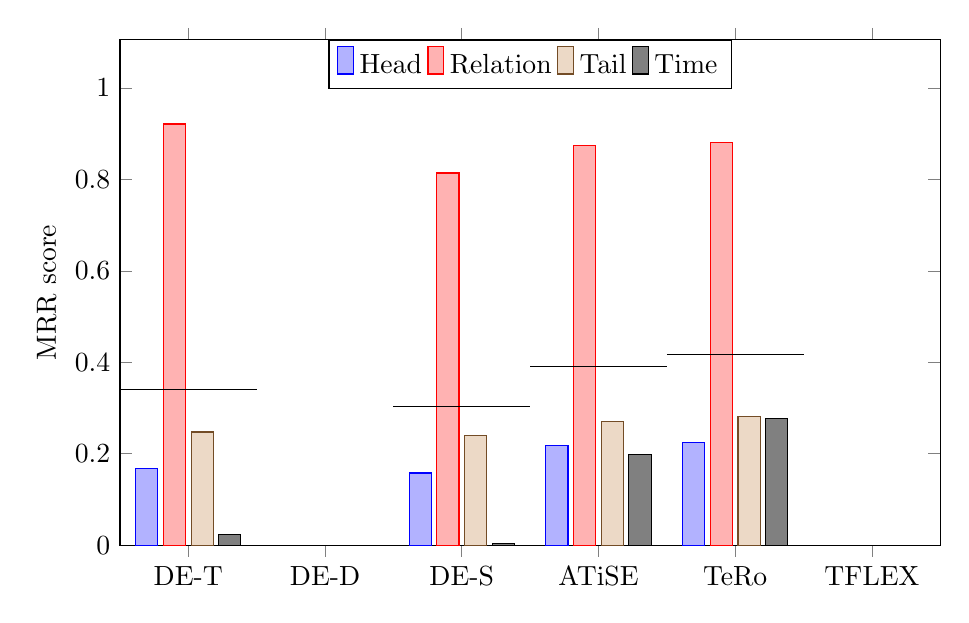
\begin{tikzpicture}
\begin{axis}[
    ybar,
    bar width=8pt,
    xticklabels={x,DE-T,DE-D,DE-S,ATiSE,TeRo,TFLEX},
    ymin=0,
    ymax=1.1055519622990757,
    ylabel={MRR score},
    height=8cm,
    width=12cm,
    legend style={
        at={(0.5,1.0)},
        anchor=north,
        legend columns=-1
    },
    legend image code/.code={
        \draw [#1] (0cm,-0.1cm) rectangle (0.2cm,0.25cm); },
    ]
\addplot coordinates { %head
(0, 0.16856201354681669) %DE_TransE
(1, 0) %DE_DistMult
(2, 0.1579443106395794) %DE_SimplE
(3, 0.21749963399555997) %ATISE
(4, 0.22541330553169855) %TERO
(5, 0) %TFLEX
} ;
\addplot coordinates { %relation
(0, 0.9212933019158965) %DE_TransE
(1, 0) %DE_DistMult
(2, 0.8141468781135313) %DE_SimplE
(3, 0.8733535658464987) %ATISE
(4, 0.8817203020512926) %TERO
(5, 0) %TFLEX
} ;
\addplot coordinates { %tail
(0, 0.24762086236479688) %DE_TransE
(1, 0) %DE_DistMult
(2, 0.24033615678654172) %DE_SimplE
(3, 0.2709493075129491) %ATISE
(4, 0.2820865071981324) %TERO
(5, 0) %TFLEX
} ;
\addplot coordinates { %time_from
(0, 0.023727251121544404) %DE_TransE
(1, 0) %DE_DistMult
(2, 0.004434572351919235) %DE_SimplE
(3, 0.19870801166124544) %ATISE
(4, 0.2779541232922569) %TERO
(5, 0) %TFLEX
} ;
\addplot[black,sharp plot,update limits=false,] coordinates { %DE_TransE
(-0.5, 0.34030085723726033)
(0.5, 0.34030085723726033)
} ;
\addplot[black,sharp plot,update limits=false,] coordinates { %DE_DistMult
(0.5, 0)
(1.5, 0)
} ;
\addplot[black,sharp plot,update limits=false,] coordinates { %DE_SimplE
(1.5, 0.30421547947288957)
(2.5, 0.30421547947288957)
} ;
\addplot[black,sharp plot,update limits=false,] coordinates { %ATISE
(2.5, 0.3901276297540677)
(3.5, 0.3901276297540677)
} ;
\addplot[black,sharp plot,update limits=false,] coordinates { %TERO
(3.5, 0.4167935595183541)
(4.5, 0.4167935595183541)
} ;
\addplot[black,sharp plot,update limits=false,] coordinates { %TFLEX
(4.5, 0)
(5.5, 0)
} ;
\legend{Head,Relation,Tail,Time}
\end{axis}
\end{tikzpicture}
\caption{wikidata12k, split 3}
\label{fig:compare_wikidata12k_3}
\end{minipage}
\end{figure*}
